\section{Algorithm Design}
\label{sec:design}

In this section, we introduce the design of the algorithm. We first present the problem formulation. Then, we present an overview of its structure. Finally we present a detailed description of its components and related algorithms.


\subsection{The Problem Formulation}
\label{problemformulation}

The key problem we are considering for the storage provisioning is to develop a sufficient, yet not wasteful, set of storage allocations from existing hardware for objects to be stored, so that applications can meet their desired performance. This problem of storage allocation is challenging due to: (1) the dynamics of workload, (2) the requirement of users, e.g., no replicas should be stored on the same rack for reliability, etc. and 3) difficulty and overhead of deriving the storage allocation results for each workload and user requirement combination. As
a result, it is difficult to determine the storage allocation that will
achieve the desired quality of service while minimizing the hardware cost and storage overhead. Therefore, if we model such a problem as a search problem whose solution is from a very large search space, then it is very hard to always reach the optimal configuration when something changes, even such change could be slight.
%
%In most cases we can resort to offline algorithms, where the results are calculated and used for a rather long period of time in storage services. This of course leads to underwhelming performance and storage waste. The key issue with existing solutions is that they do not handle dynamics in the requests or workloads successfully. Moreover, on-line algorithms may not be fully predictable in their convergence time, leading to long delays and out-of-date solutions. This problem may become even worse when different types of hardware such as SSD is used, or servers may be added or removed due to failures, and so on.

Based on such concerns, we formulate the following problem: \textbf{given the underlying demands, how can we find an optimized storage placement that can incrementally provide results that can achieve the best performance under the resource constraints and user requirements?} Note that given that the users' request may change frequently, we would like to be able to re-use previous calculation results as much as possible, so that we can avoid the re-calculation when a similar scenario is met in practice.

\begin{figure}[t]
\begin{centering}
  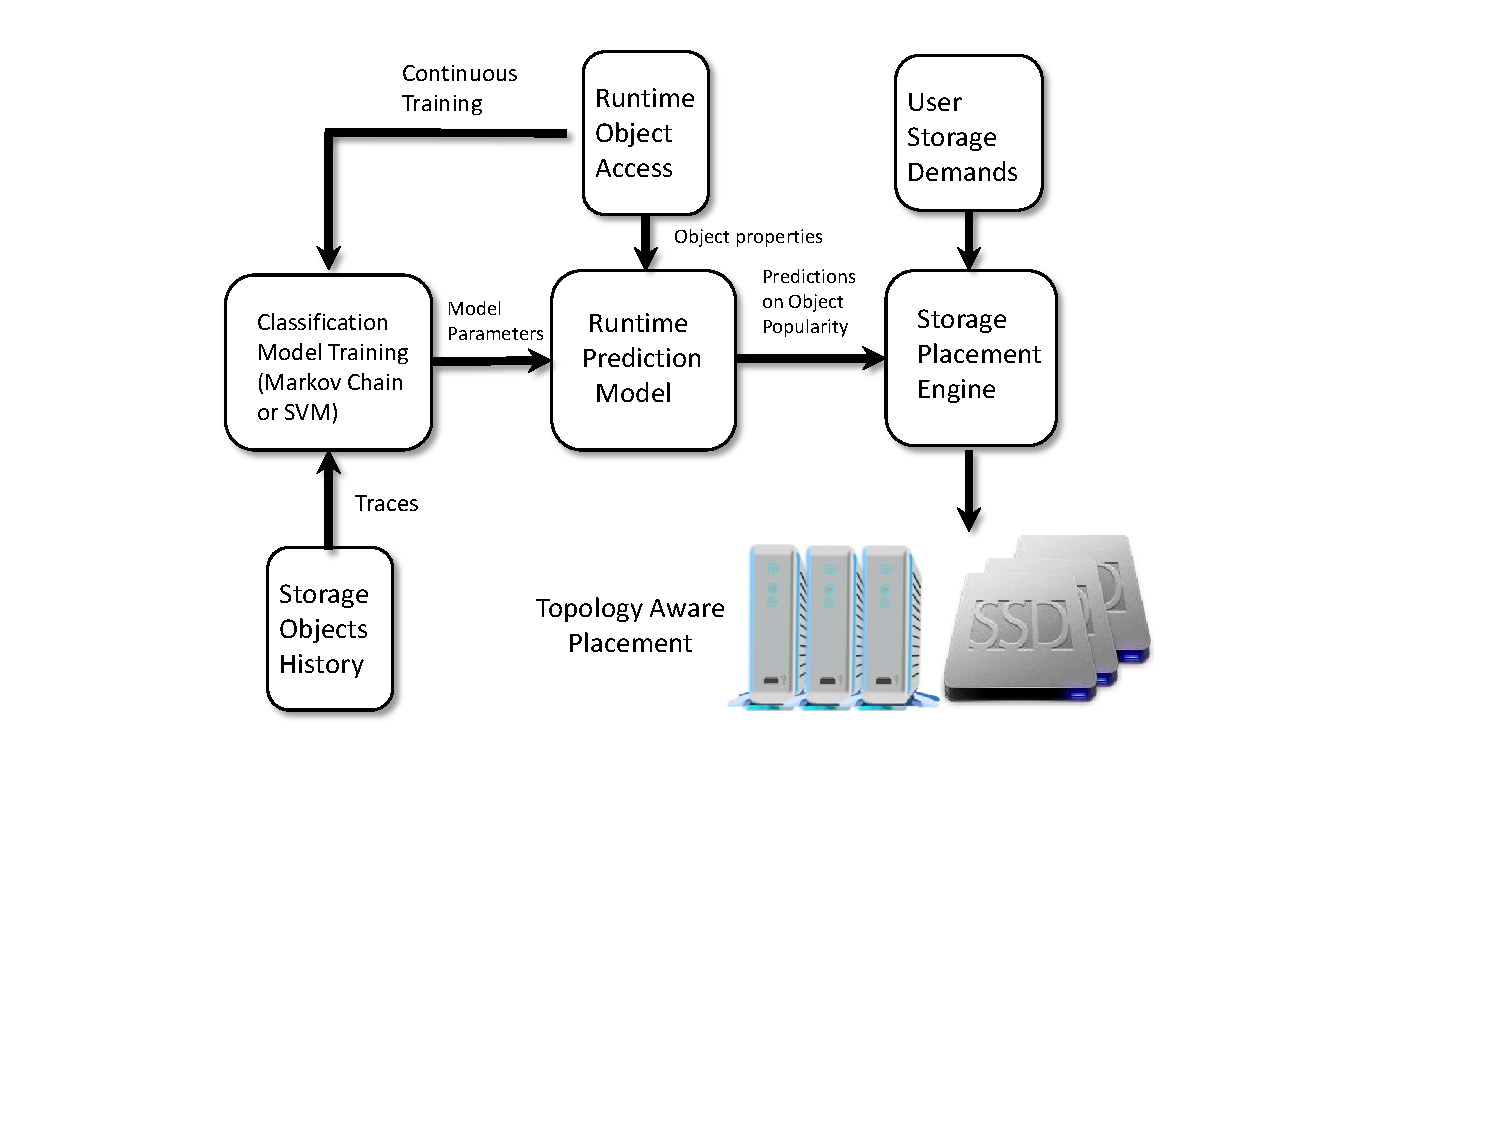
\includegraphics[width=3.3in]{./ModelPhase.pdf}
  \caption{The architecture of workflow}\label{fig:architecture}
  \label{arch}
\end{centering}
\vspace{-0.1in}
\end{figure}


\subsection{Architecture Overview}
\label{architecture}

Figure~\ref{arch} shows the overall architecture of the proposed workflow, where the whole procedure works as follows:  the first core component, the classification model, is trained based on the access history of storage objects. It then provides the model parameters for the runtime prediction model, which is used to classify runtime access to objects. Such accesses are classified into either ``recurring'' or ``non-recurring'', depending on whether the objects are considered to be popular or not. The popularity metric for objects, as well as the user storage demands, are then handled by the storage placement engine to move storage objects as needed. Note that such placement of data can be either on the hard disks or SSDs, depending on users' requirements. Finally, the runtime object access traces are also used as input for the classification model for continuous training purposes.


\subsection{Design Assumptions}

We now present our design assumptions. We assume that the user of the service deploys their service across a pool of storage servers. The storage servers could be a set of OSDs, which are intelligent controllers that can map the requests from the user to the storage services. Each of the OSD may provide some level of SLO (Service Level Objective) for the deployed service.

During the system's operation, we assume that users' requests include both reading and writing operations. Note that the writing operations may be dominating for certain workflows, such as checkpoint backups that require periodic operations~\cite{}. The users' workloads may also change over time, which requires that the system should adapt to the requirements and demands.



\subsection{Learning based Workload Classification}

In this section, we describe how the classification model generates model parameters based on storage object history traces. Specifically, once the features are selected, we then collect training data for a period of time. The task then becomes a classification problem, where we need to evaluate the effect of selected features on classification accuracy. In our design, we adopt a Markov chain based approach. More specifically, suppose that we select $N$-tuple that forms a workload signature as:

\[
  Signature = {m^1, m^2, ..., m^n}
\]

where the $m_i$ represents a measured metric of $i$. Note that the metric selection process is fully automated and transparent to the user.

Once the signatures are collected, it is important that we can classify later workloads based on the training periods. This is based on the assumption that user workloads will have inherent repeating patterns, where similar workloads may be encountered again. This therefore resembles the ``cache hit rates'' which are well studied in the computer cache designs. But still there are considerable differences, as unlike cache contents, the workload signatures may indeed shift over time. Therefore, it is only giving approximate solutions, not accurate answers.

Note that there is a tradeoff in the overhead of training and prediction and the achieved hit rates. We need to achieve a good tradeoff in this design. We make the following assumptions regarding OSDs. First, we assume that each OSD can maintain the access history for each data object. In reality, it may not be practical to record a long access history for each data object since in that case the storage overhead could be huge, instead, only recent access history are maintained and updated periodically. Second, we model the access frequency of each data object using a discrete-time Markov chain in which each state represents a specific range of access frequency. With the access history, we can estimate the parameters of the Markov chain model. Third, by calculating the stationary distribution of the Markov chain, we can predict how possible the access frequency of each data object lies within certain range in the long run. Finally, we rank each data object based on the weighted sum of the stationary distribution and the weights are chosen according to the specific range represented by each state in the Markov chain. The highest rank the data object has, the more possible it will be moved to SSD devices.

\subsubsection{Access History of Data Objects Collection}

Fig. \ref{trace} demonstrates the access frequency (Here the ``access'' includes both reads and writes.) of a data object during one month.  The x axis of Fig. \ref{trace} is the range of one month time which has been divided into 720 sections (each section is 1 hour) and each point on x axis represents each of these time sections. The y axis represents the number of times the data object has been accessed during each time section.

\begin{figure}[!t]
\centering
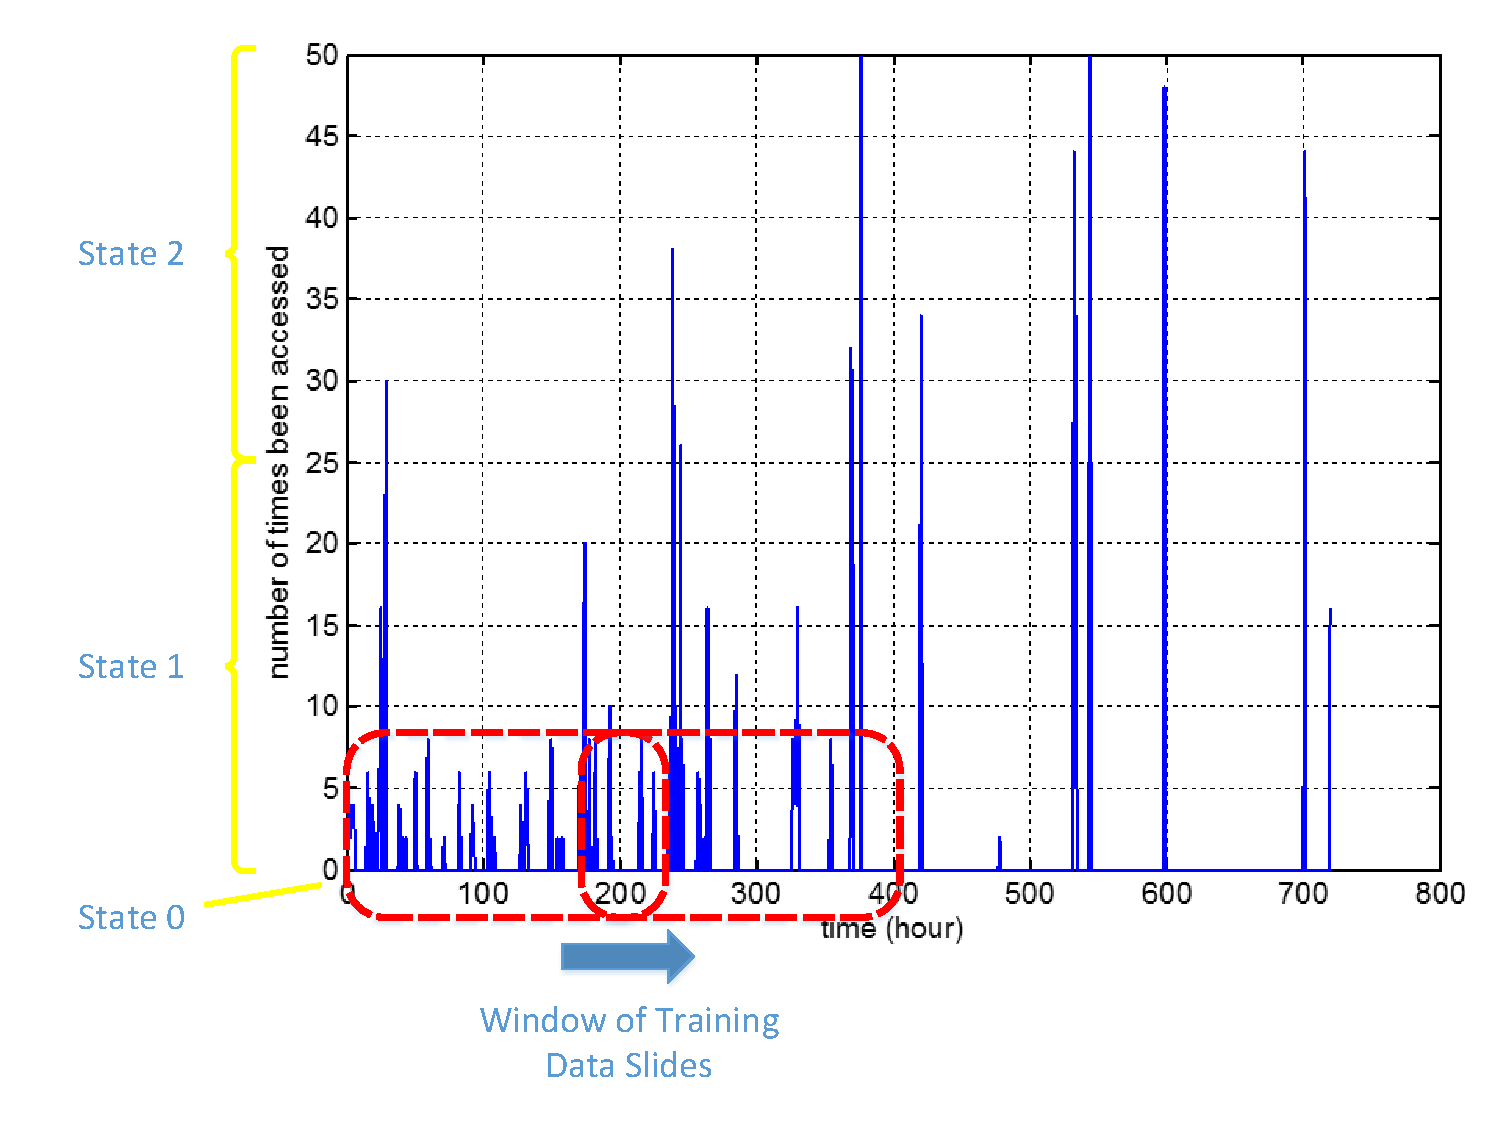
\includegraphics[width=3.0in]{./trace.pdf}
% where an .eps filename suffix will be assumed under latex,
% and a .pdf suffix will be assumed for pdflatex; or what has been declared
% via \DeclareGraphicsExtensions.
\caption{Trace of Data Object Access Frequency}
\vspace{-0.25in}
\label{trace}
\end{figure}

As we mentioned at the beginning of this section, since the storage overhead, maintaining the entire access history of each data object on each OSD is not acceptable. Thus, we only maintain recent access history of each data object and use such access history to build a Markov chain model to predict the future access frequency. As shown in Fig. \ref{trace}, only the access history in the window which has red dot borderline is used to train the prediction model and the window of training data slides with time so that we can implement online prediction for data objects access frequency.

\subsubsection{Markov Chain Predication Model}

With the access history of each data object, we can now build the Markov chain model to predict the future access frequency of data objects. First, we need to determine how many states the Markov chain should have and the range of access frequency each state represents. For example, as shown in Fig. \ref{trace}, if the maximum number of access times during an observation period is 50, then we can divide 50 evenly and build a Markov chain model that has 3 states. If during a time section, there is no access of the data object, then the Markov chain will stay in state 0. If during a time section, the number of access times is larger than 0 but less than 25, then the Markov chain will stay in state 1, and so on. The transition diagram of the Markov chain is shown in Fig. \ref{transitioin}.

\begin{figure}[!t]
\centering
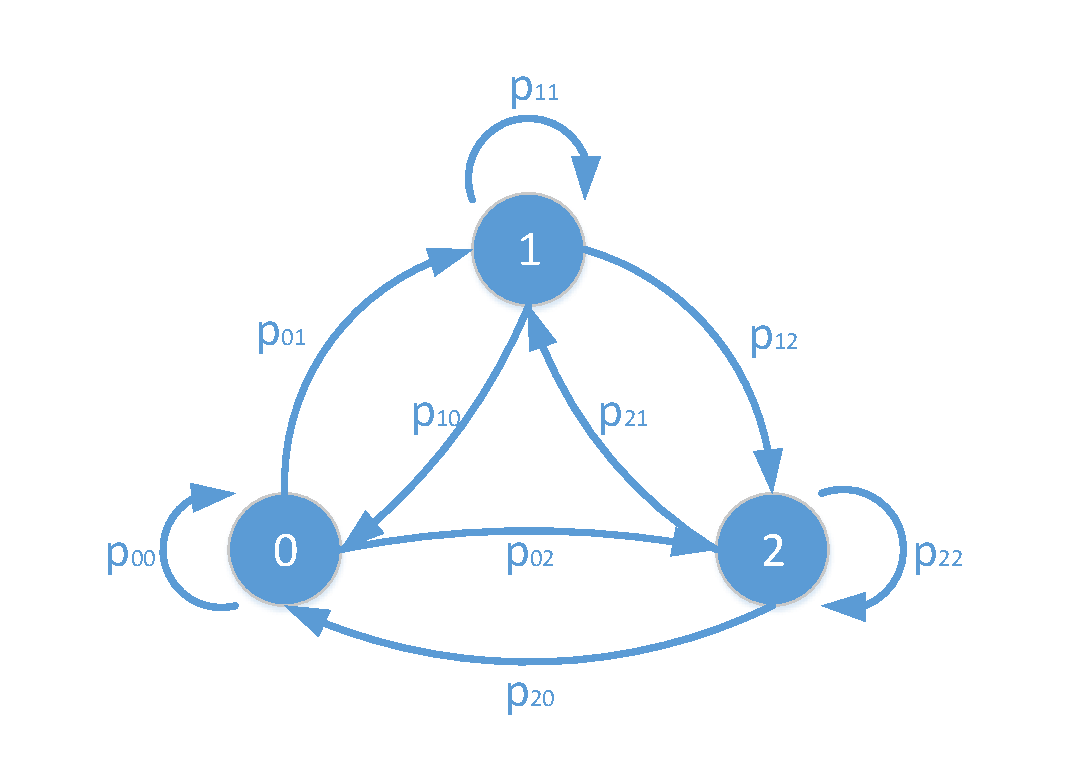
\includegraphics[width=3.0in]{./transition.pdf}
% where an .eps filename suffix will be assumed under latex,
% and a .pdf suffix will be assumed for pdflatex; or what has been declared
% via \DeclareGraphicsExtensions.
\caption{Transition Diagram of Markov Chain}
\vspace{-0.25in}
\label{transitioin}
\end{figure}

Second, we transform the access history to the state transition sequence of the Markov chain based on the specific range each state represents. For example, after transformation the state transition sequence of access history shown in Fig. \ref{trace} is: 1,1,1,1,1,0,0,... Based on the state transition sequence, we can estimate the transition probabilities between every two states and construct the transition matrix of the Markov chain shown below:
\begin{equation}
\mathbf{T} =
 \begin{pmatrix}
  p_{00} & p_{01} & p_{02} \\
  p_{10} & p_{11} & p_{12} \\
  p_{20} & p_{21} & p_{22}
 \end{pmatrix}
\end{equation}

According to the properties of Markov chain, we have:
\begin{equation}
\lim_{n\to\infty}\mathbf{T}^{n} =
 \begin{pmatrix}
  \pi_{0} & \pi_{1} & \pi_{2} \\
  \pi_{0} & \pi_{1} & \pi_{2} \\
  \pi_{0} & \pi_{1} & \pi_{2}
 \end{pmatrix}
\end{equation}
in which $\boldsymbol{\pi} = [\pi_{0}, \pi_{1},  \pi_{2}]$ is called the stationary distribution of the Markov chain. We can simply calculate $\boldsymbol{\pi} $ through computing a normalized multiple of a left eigenvector $\mathbf{e}$ of the transition matrix $\mathbf{T}$ with an eigenvalue of 1:
\begin{equation}
\boldsymbol{\pi} = \frac{\mathbf{e}}{\sum_{i}e_{i}}
\end{equation}
Since the stationary distribution $\boldsymbol{\pi}$ reflects the probabilities that each state of Markov chain will be visited in the future, which can be used to predict the access frequency of each data object.

Finally, we need to rank the data objects on an OSD based on the prediction results so that we can determine which data object should be moved to SSD devices. As different states of the Markov chain represent different access frequency ranges, they have different importance to the prediction results. For example, even if the calculated stationary distribution tells us state 1 will be visited with higher probability than state 2, to rank the importance of the data object, we must consider that state 2 represents higher access frequency. Therefore, we use a weighted sum of the stationary distribution to rank the importance of the data object and the weights are defined by values that are proportional to the access frequency ranges the states represent. For example, if we obtain the stationary distribution of the data object is $\boldsymbol{\pi} = [0.31, 0.56, 0.13]$, and we assign weights $[0, 10, 20]$ to the three different states, we can calculate the rank of the data object by $rank_{obj_{x}} = 0.31\times0+0.56\times10+0.13\times20 = 8.2$.

\subsection{Parametric User Demand Profiling}

The second novel contribution of our work is that we will adapt the storage placement based on user demands, such as the locations of redundant copies and the frequency of making duplicates, in the face of possible failures. In this aspect, we assume that users' requests will be parametric, meaning that all requests will be embedded into equations or constraints. For example, a requirement on the number of redundant copies can be expressed as $RedundantCopy > 3$.  Therefore, for the storage placement algorithm to be effective in dealing with such dynamic requirements, it first needs to receive such demands from users, and their associated storage needs. To profile a requirement, our algorithm uses a profiler that is deployed along the path of the users' requests. The profiler serves requests in the profiling environment, allowing us to collect all metrics that are needed for the characterization of users' requirements. Note that such profiling is occurring independently of the OSD servers that handle such requests concurrently.

The advantage of having the profiler operating independently of the OSDs lies in that this does not require our profiler to be tightly integrated into the rest of the system. Therefore, the profiler can be easily replaced as needed, which gives us additional flexibility.

The central task of the profiler is that it will pick the requirement one by one and fulfill them, depending on their urgency and the amount of resources needed to fulfill them. For the profiling to be most effective, it is critical to pick a set of metrics that form the bottleneck. This is based on the observation that once we fulfill one bottleneck requirement, usually more than one requirements will be met. 
 
Ideally, the collected metrics for the incoming workloads should allow us to uniquely find a placement of storage OSDs without the details of the workloads themselves. This is because the algorithm is by nature greedy, and in the worst case, it will traverse all possible requirements from the user and fulfill them. 
